
\capitulo{SISTEMA DESENVOLVIDO}

\iniciocapitulo
O capítulo descreve o sistema desenvolvido neste trabalho, tem como objetivo o sistema, otimizar a alocação das disciplinas envidas pelos colegiados em salas de uma universidade, neste caso as salas do prédio FAFICH na UFMG. Por se tratar de um problema especifico do local torna-se difícil o trabalho de encontrar tecnologias disponíveis para otimização do problema, neste caso o desenvolvimento de um sistema que atenda todas as necessidades é de grande importância para o responsável pela alocação.\par

\secao{Modelagem}

\subsecao{Diagramas de caso de uso}

A Figura XX descreve todas as funcionalidades que o sistema possui, essas funcionalidades foram dividias em 2 atores "Gerente" e "Sistema" cada um ligado com suas respectivas funcionalidades, porem, o "Gerente" pode acessar o ator "Sistema" para ter acessos funcionalidades que são encontradas no mesmo. O sentido das setas informa o que cada ator pode acessar no sistema.\par

As funcionalidades controle de turnos, controle de horários, controle de prédios, controle de salas, controle de cursos, controle de colegiados, controle de períodos e controle de disciplinas são disponibilizadas através de módulos CRUD para que o responsável tenha total controle sobre o que será alocado, onde e como.\par

Já as funcionalidades alocação de horários e geração de relatórios, são rotinas executadas pelo "Sistema". A funcionalidade alocação de horários é uma rotina que utiliza conceitos de algorítimo genético para encontrar a melhor solução do problema e a funcionalidade geração de relatórios mostra para o "Gerente" o melhor resultado de alocação encontrado pelo algorítimo.\par

\begin{figure}[!htb]
\caption[Diagrama de Caso de Uso]{Diagrama de Caso de Uso}
\label{fig:figura1}
\centering
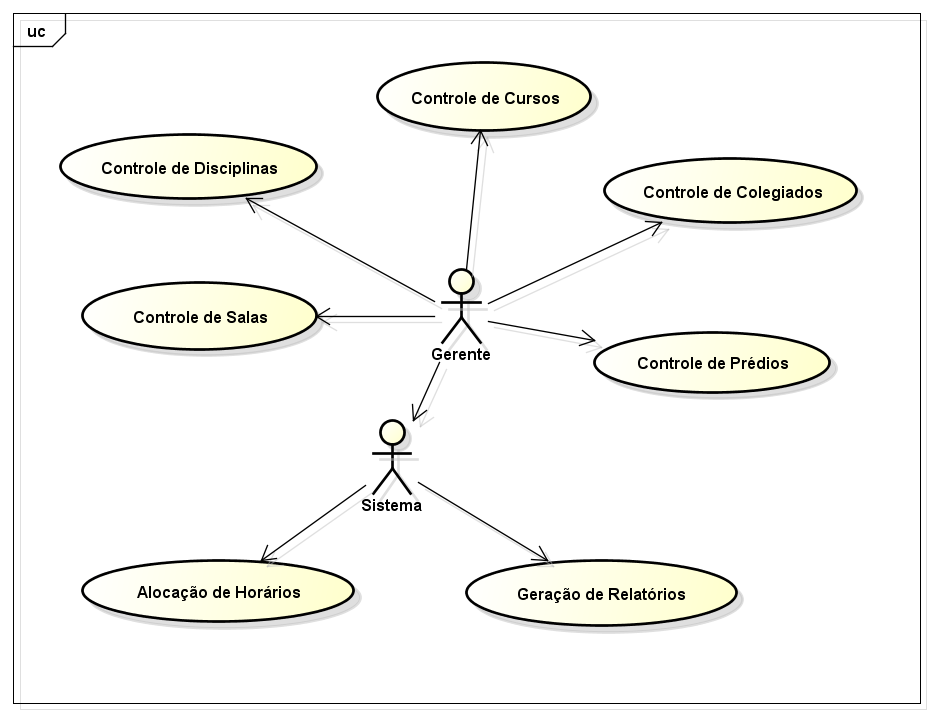
\includegraphics[scale=0.4]{imagens/diagramaCasoUso.png}
\\ \textbf{\footnotesize Fonte: Desenvolvido pelo autor}
\end{figure}

\subsecao{Diagrama de Entidade Relacionamento}

Na Figura XX mostra o relacionamento das tabelas no sistema atraves do diagrama de entidade relacionamento.\par

As tabelas curso, colegiado, período, disciplina, sala, prédio, turno, horário são utilizadas para armazenar as informações dos respectivos objetos que são controlados pelo CRUD e suas respectivas funcionalidades.\par

A tabela relacionamento\_disciplina\_horário, salva as obrigatoriedades dos horários das disciplinas uma vez que todos os horários são montados pelos colegiados e não pelo responsável pela alocação das disciplinas nas salas.\par

A tabela alocação contem o relacionamento de disciplina, horário e sala o que corresponde a melhor alocação encontrada pelo algorítimo. O item disciplina pode ter o seu valor como nulo o que significa que em um especifico horário e em uma determinada sala não existe disciplina alocada.\par

A tabela parâmetro é utilizada apenas para guardar os últimos parâmetros utilizados na execução do algorítimo genético.\par

\begin{figure}[!htb]
\caption[Diagrama de Entidade Relacionamento]{Diagrama de Entidade Relacionamento}
\label{fig:figura2}
\centering
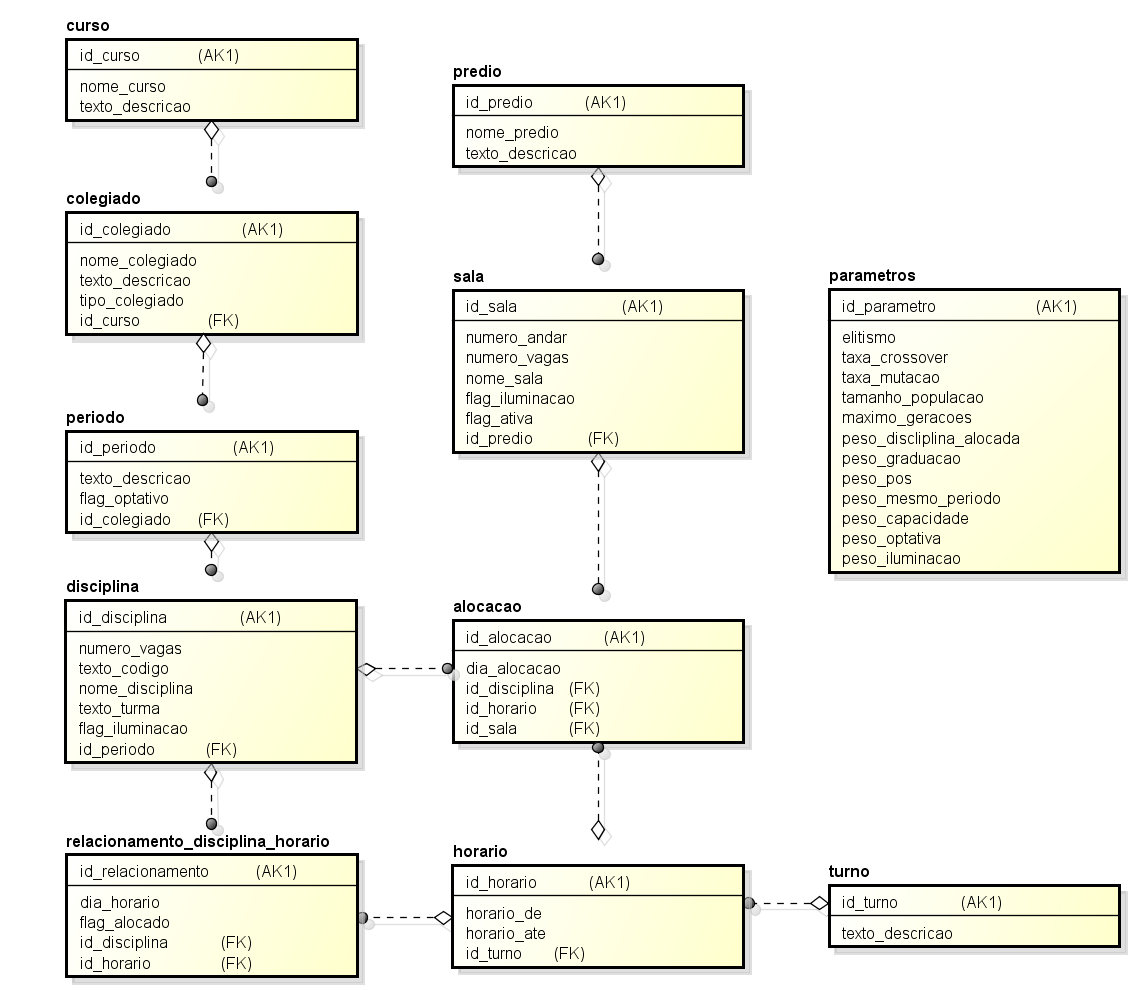
\includegraphics[scale=0.5]{imagens/diagramaEntidadeRelacionamento.png}
\\ \textbf{\footnotesize Fonte: Desenvolvido pelo autor}
\end{figure}

\subsecao{Diagramas de classe}

Este diagrama é das classes do algorítimo genético, as classes do sistema em geral não serão abordados. Quando terminar o codigo revisar e explicar.\par
Lorem ipsum dolor sit amet, consectetur adipiscing elit. Donec vestibulum mauris at velit varius aliquet. Nulla at risus vehicula, tempus orci sagittis, molestie nibh. Fusce sodales sollicitudin viverra. Aliquam erat volutpat. Nullam nec odio mi. Suspendisse vel mauris felis. In mi diam, auctor vel feugiat ut, pulvinar ac ipsum. In a convallis arcu. Integer a augue accue rutrum mauris. Phasellus id massa a lorem semper placerat eget eu urna.\par

\begin{figure}[!htb]
\caption[Diagrama de Classe]{Diagrama de Classe}
\label{fig:figura3}
\centering
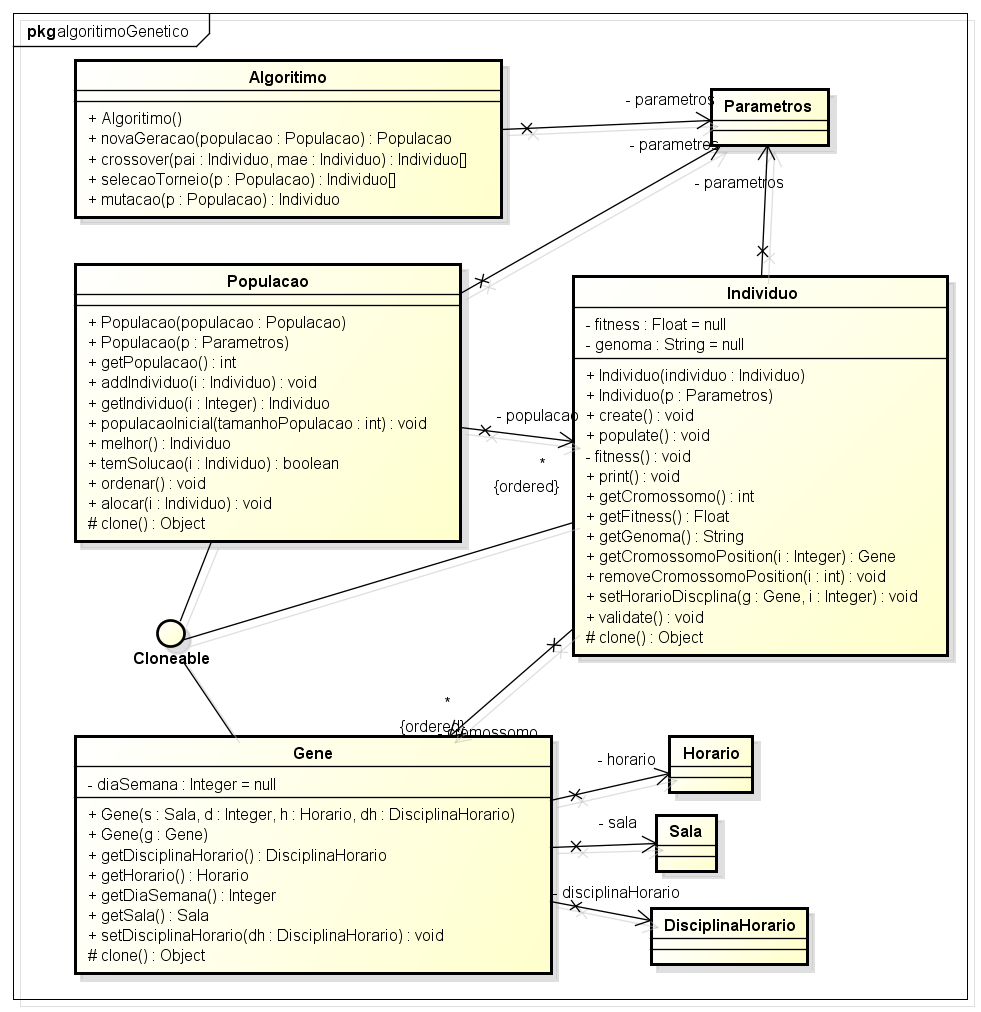
\includegraphics[scale=0.6]{imagens/diagramaClasse.png}
\\ \textbf{\footnotesize Fonte: Desenvolvido pelo autor}
\end{figure}

\secao{Algorítimo Genético}

Após a execução da modelagem do sistema com pleno conhecimento do problema e o levantamento bibliográfico sobre algorítimos genéticos, foi feito o relacionamento do problema com os termos da biologia. Foram encontradas varias fontes que agregaram valor para o desenvolvimento do trabalho, porem algumas modificação foram feitas para que o modelo tratado por outros autores funcionasse adequadamente para a resolução do problema proposto para este trabalho. A seguir serão apresentados os itens da biologia utilizados no desenvolvimento do algorítimo juntamente com sua ligação com o problema.\par

\subsecao{Indivíduo}

Alguns trabalhos tratam os termos indivíduo e cromossomo como a mesma representação biológica, neste trabalho o termo indivíduo é composto pelo cromossomo juntamente com a pontuação adquirida após a execução do método de calculo de fitness, já o termo cromossomo se refere a combinação dos genes do indivíduo, a figura XX demonstra a representação de um indivíduo.\par

\begin{figure}[!htb]
\caption[Representação Individuo]{Representação Individuo}
\label{fig:figura7}
\centering
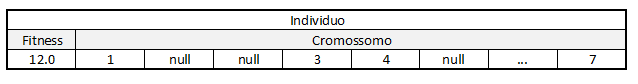
\includegraphics[scale=0.8]{imagens/representacaoIndividuo.png}
\\ \textbf{\footnotesize Fonte: Desenvolvido pelo autor}
\end{figure}

Um cromossomo é uma sequência de genes, neste trabalho esta sequência tem um tamanho fixo e pode ser medido pela seguinte formula (número de Salas * número de Horários * número de dias da semana). Inicialmente o individuo contem todos as variáveis relacionamentos de obrigatoriedade nulas, estas variáveis serão preenchidas randomicamente na criação da população inicial que em breve será explicada. O cromossomo do indivíduo preenchido com os relacionamentos de obrigatoriedades representa uma alocação, está alocação é medida pela sua pontuação de fitness, podendo ser ou não o resultado do problema. Os valores utilizados na representação do cromossomo na figura XX são os ID's do relacionamento de obrigatoriedade entre horário e disciplina, em caso de horário vago em um determinado gene esta variável terá o valor nulo.\par

\begin{figure}[!htb]
\caption[Representação Cromossomo]{Representação Cromossomo}
\label{fig:figura6}
\centering
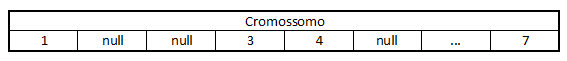
\includegraphics[scale=0.9]{imagens/representacaoCromossomo.png}
\\ \textbf{\footnotesize Fonte: Desenvolvido pelo autor}
\end{figure}

O termo gene representado pela figura XX possui uma combinação de quatro variáveis sala, dia da semana, horário e o relacionamento de obrigatoriedade 
"disciplina horário". As variáveis sala, horário e dia da semana são fixas, não podem ser nulas uma vez que todas as combinações possíveis destas três variáveis formam um cromossomo que tem um tamanho fixo para todos os indivíduos. \par

Um gene com o relacionamento "disciplina horário" igual a nulo, representa um horário vago para aquela combinação especifica de sala, horário e dia da semana.\par

\begin{figure}[!htb]
\caption[Representação Gene]{Representação Gene}
\label{fig:figura5}
\centering
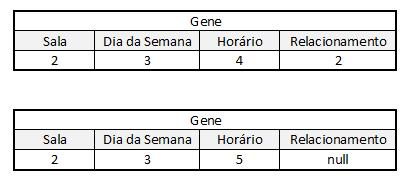
\includegraphics[scale=0.7]{imagens/representacaoGene.png}
\\ \textbf{\footnotesize Fonte: Desenvolvido pelo autor}
\end{figure}

O fitness do indivíduo é calculo através da função objetivo que será abordada em outro tópico brevemente explicando se trada de um valor que vai de 0 a 100 onde 100 é a pontuação máxima de do indivíduo está nota é alcançada quando todos os requisitos de alocação desejados foram atendidos.

\subsecao{População}

Uma população, quando relacionada aos termos genéticos se trata de um conjunto de indivíduos, também representa uma interação do algorítimo genético, ou seja uma geração.A manipulação da população e de suas propriedades é feita através de parâmetros enviados antes da execução do algorítimo, estes parâmetros são elitismo, taxa de crossover, taxa de mutação, tamanho da população e número máximo de gerações.

De acordo com os parâmetros passados é criada a população inicial. Para cada indivíduo criado é utilizado um método para inserir randomicamente todos os registros de relacionamento de obrigatoriedade entre disciplina e horário em cada um dos genes que previamente foram criados como nulo, estes indivíduos são criados até a população atinga o tamanho da população que deve ser igual ao parâmetro tamanho da população.\par

Para cada geração é criada uma nova população a partir da população criada na geração anterior, se o operador genético elitismo estiver como valor verdadeiro, iniciamos está nova população com 20\% dos melhores indivíduos da população anterior, os melhores indivíduos de uma População são indicados pelas maiores pontuações de fitness de da população anterior.\par

Durante a criação da nova população podemos ter duas operações ocorrendo mutação e crossover, para a execução destes operadores genéticos são utilizadas porcentagens enviadas pelos parâmetros do algorítimo. Para que estas operações genéticas aconteçam são utilizados valores randomicos para serem comparados com as taxas de mutação e crossover. Em cada interação da criação desta nova população são selecionados por torneio os pais que serão utilizados no crossover, se a condição da taxa de execução for verdadeira os pais serão descartados e os filhos gerados a partir dos genes dos pais, serão adicionados na nova população, em caso de falso os pais serão adicionados na nova população.\par
Para se utilizar a operação de mutação novamente é utilizado outro valor randominco se a condição for verdadeira um indivíduo da população anterior é selecionado e sofrerá a mutação genética, o individuo antes da mutação genética é descartado e o novo indivíduo que sofreu a mutação é adicionado na nova população. O fluxo de uma nova população é descrito na figura XX.\par

\begin{figure}[!htb]
\caption[Fluxo Nova População]{Fluxo Nova População}
\label{fig:figura8}
\centering
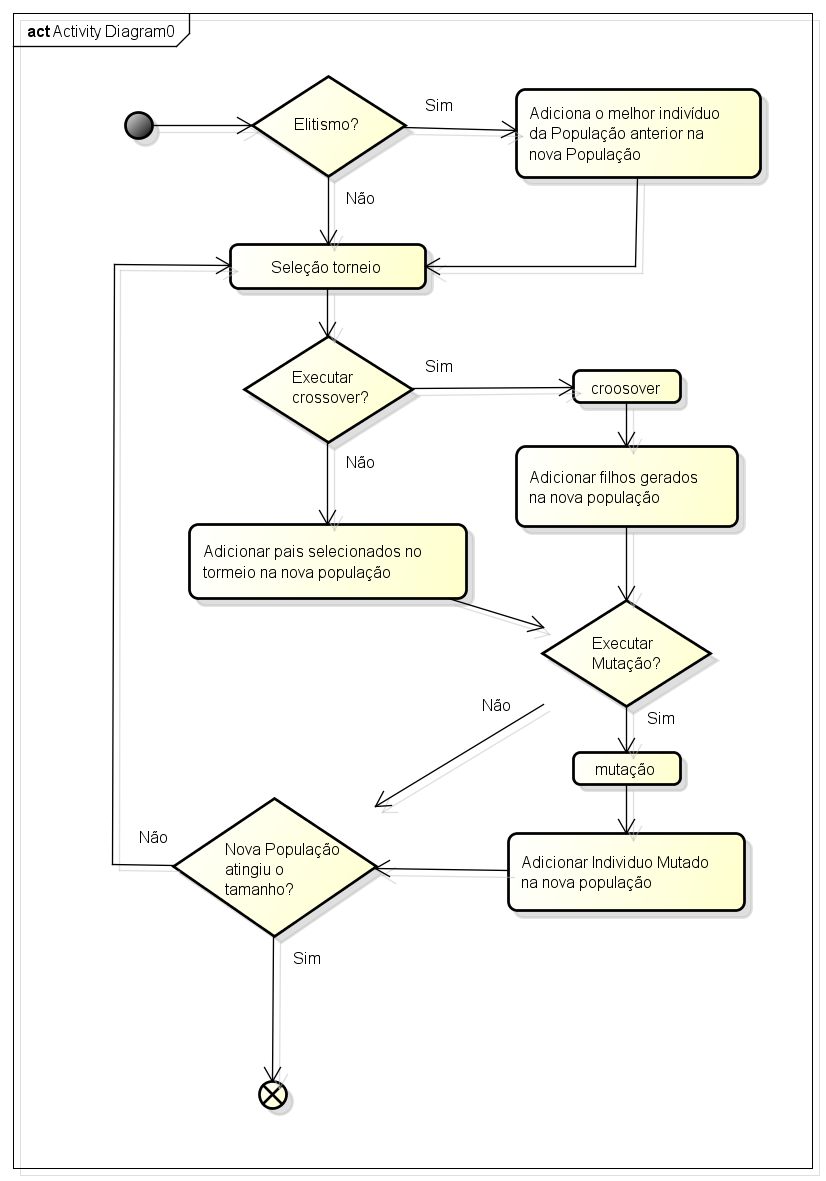
\includegraphics[scale=0.7]{imagens/fluxoNovaPopulacao.png}
\\ \textbf{\footnotesize Fonte: Desenvolvido pelo autor}
\end{figure}

\subsecao{Operadores genéticos}

Este trabalho utiliza elitismo como operador genético ao se inciar uma nova população, vinte porcento dos melhores indivíduos são escolhidos para compor a nova população.O elitismo é calculdo atravez da função objetiva criada para o problema especifico do trabalho.\par

Para selecionar os inviduos para realizar o crossover é utilizado metodo de seleção por torneio, são escolhidos três Individuos da população anterior, e destes três são escolhidos os dois com maior pountuação de fitness, os dois Individuos selecionados são enviados para o crossover.\par

Mutacao é a inversão genetica dos genes de um Individuo escolhido randomicamente da população anterior, apos a realização da mutação genetica o individuo é inserido na nova população.\par

Primeiramente são escolhidos dois genes do cromossomo, apos a escolha randomica dos itens a serem trocados, é feita a troca dos genes e retornado um ndividuo que tem a composição genetica apos a alteração, Apos a mutação este Individuo recebe uma nova nota de fitness de acordo com a sua nova sequencia de Genes e sua adaptação no ambiente, está nota pode ser maior ou menor do que a anterior.\par

\begin{figure}[!htb]
\caption[Representação Mutação]{Representação Mutação}
\label{fig:figura8}
\centering
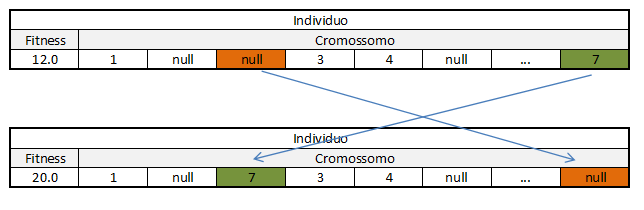
\includegraphics[scale=0.7]{imagens/representacaoMutacao.png}
\\ \textbf{\footnotesize Fonte: Desenvolvido pelo autor}
\end{figure}

Crossover é o cruzamento dos individuos selecionados pela seleção torneio. Explicar com figuras. apos o cruzamento dos individuo os dois filhos gerados são inseridos na nova população.\par

\subsecao{Definição da função objetivo}

Somatorio disso

Para o calculo do fitness foram definidos pesos para modelagem da função, estes pesos podem ser configurados de acordo com a necessidade da alocação.

Graduação alocada ganha 05 de peso

Pós graduação alocada ganha 03 de peso

Periodos na mesma sala cada um ganha 05 de peso * o numero do periodo

Quanditadade de vagas igual a da sala 05 de peso

não optativa ganha 5

optativa ganha 3

iliminacao atendida 5

Criar a função matematica com as legendas conforme o trabalho 117.pdf

Falar o numero de salas, o numero de horarios, o numero de curos o numero de colegiados o numero de periodos o numero de disciplinas para cada colegiado.......

restrições 


falar um pouco das restrições e enumeralas

As disciplinas não podem ser alocadas em horarios direfentes dos que já foram pré definidos pelo colegiado.

As discplinas devem ter apenas a quantidade de alocações necessarias.

As disciplinas devem respeitar a capacidade da sala.

As diciplinas não optativas tem preferencia de alcação na mesma sala.

Preferencias por salas claras ou escuras

Restrição 1 


Fitness

Para se iniciar o calculo do fitness são verificados todos os horarios já alocados somando os pesos se adequados.

para cada gene

se tem horario alocado 

horario bate

capacidade da turma

turma graduacao

optativa

iluminacao

soma tudo

fim se tem alocação

soma tudo

fim para cada gene

Calculo do fitness01 somatatoriox100/colocar algum valor  para dividir não sei ainda

calculo fitness02 penaliza disciplinas com mais alocação do que se deve

para cada gene 

para cada disciplina 

soma

fim

Calculo fitness02 -= fitnes01 x (1 - (total alocados - total necessario/ dividir pelo numero possivel de alocações))
fim

calculo fitness03 penalidade por capacidade

para cada gente

se a sala tiver capacidade diferente

fim

calculo fitness03 = fitness02 x (1 - (numero de erros /  numero de possiveis alocações )))


calculo fitness04 preferencias clara ou escura

para cada gene 

se tiver com o optativo errado 

fim	

calculo fitness04 = fitness03 x (1 - (numero de erros /  numero de possiveis alocações )))


O fitness04 é o resultado final

\subsecao{Fluxo do algoritimo}

parametros Algoritimo

O fluxo do algorimo conforme a imagem XX é iniciado pela criação da população inicial, para cada interação do algoritimo é verificado se a população contem o resultado e se o algoritimo não atingiu o numero de gerações pré defindas. Se as duas condições forem falsas o algoritimo cria uma nova População de acordo coma figura XX

\begin{figure}[!htb]
\caption[Fluxo Algoritimo]{Fluxo Algoritimo}
\label{fig:figura8}
\centering
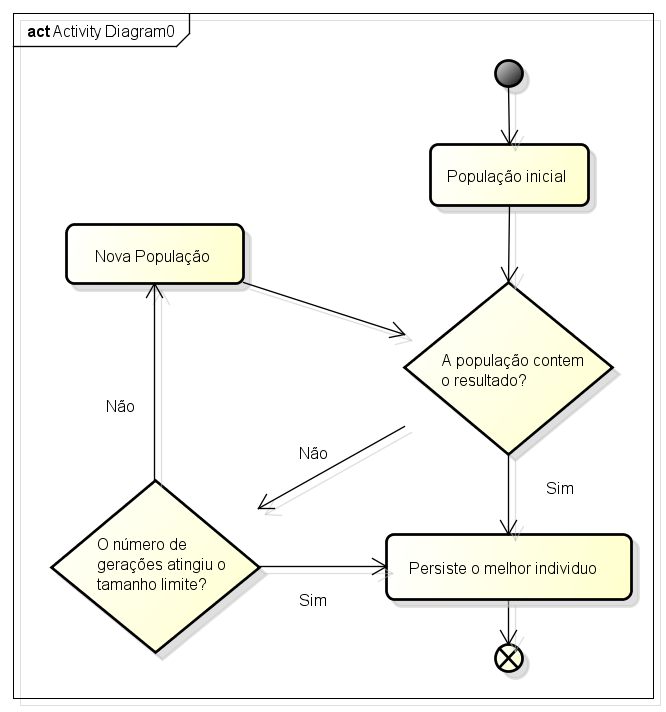
\includegraphics[scale=0.7]{imagens/fluxoAlgoritimo.png}
\\ \textbf{\footnotesize Fonte: Desenvolvido pelo autor}
\end{figure}